\documentclass[11pt]{article}
%\renewcommand{\thesection}{\Roman{section}}  %zmiana section na rzymskie
\usepackage[utf8]{inputenc}
\usepackage[OT4]{polski}
\usepackage{tabularx}
\usepackage[margin=60pt]{geometry}
\usepackage{amsmath}
\usepackage{amsfonts}
\usepackage{listings} 
\usepackage[usenames,dvipsnames,table,xcdraw]{xcolor}
\usepackage{array}
\usepackage{sidecap} %do grafik
\usepackage{wrapfig} % j. w.
\usepackage{graphicx} %j.. w.
\usepackage{subfig} %j. w.
\usepackage{booktabs}
\usepackage{longtable}
\usepackage{hyperref}
\usepackage{multirow}



\title{Obliczanie rozkładu potencjału elektrostatycznego w nanostrukturze półprzewodnikowej
wykorzystywanej przy budowie tzw. elektrostatycznych kropek kwantowych.}

\author{Paweł Rzońca}

\begin{document}

\maketitle

\section*{Wstęp}
Ćwiczenie polegało na zamodelowaniu rozkładu potencjału wewnątrz nanourządzenia stanowiącego elektrostatyczną kropkę kwantową. Zagadnienie
sprowadza się do rozwiązania równania Laplace'a (\ref{rowL}) przy odpowiednich warunkach brzegowych. 
\begin{equation}
\nabla^2 \varphi (x,y,z) = 0 \label{rowL}.
\end{equation}
Warunki brzegowe zadajemy jako zerowanie się pochodnej na brzegach pudła obliczeniowego. We wnętrzu rozmieszczamy płaskie elektrody (Rys. \ref{ele}) 
na których ustalamy stały potencjał. Dodatkowo uziemiamy dolną powierzchnię. 
\section*{Metodyka}
Równanie Laplace’a rozwiązujemy rozwiązać iteracyjnie osiągając tzw. samouzgodnenie. 
Wykorzystujemy wzór 
\begin{equation}
\begin{aligned}
\varphi_{n+1} (x,y,z) = \dfrac{1}{2/(\Delta x)^2 + 2/(\Delta y)^2 + 2/(\Delta z)^2} \left[ \dfrac{\varphi_n (x + \Delta x,y,z) + 
	\varphi_n (x-\Delta x,y,z)}{(\Delta x)^2} \right. + \\
	+ \left. \dfrac{\varphi_n (x,y+\Delta y,z) + \varphi(x,y-\Delta y,z)}{(\Delta y)^2} + \dfrac{\varphi_n(x,y,z+\Delta z)+
	\varphi_n (x,y,z-\Delta z)}{(\Delta z)^2}  \right].
\end{aligned}
\end{equation}
Na powierzchni podłoża ustalamy wartość potencjału, przyjmiemy potencjał ujemny $V_0$=-350 mV. Na czterech elektrodach narożnych przyjmiemy
$V_1=V_2=V_5=V_6=450$ mV, a na obu środkowych $V_3=V_4=300$ mV. Na wszystkich pozostałych ścianach prostopadłościanu przyjmiemy zerowanie się pochodnej
normalnej do powierzchni, tj. wartości na brzegach przyrównujemy do wartości tuż przed brzegiem. Warunki te są słuszne dla odpowiednio dużej odległości
od elektrod (w idealnym przypadku nieskończonej). Z tego powodu sprawdzamy dla jakich $nz$ (wysokości pudła) wysokość potencjału wewnątrz studni
nie zmienia się przy dalszym zwiększaniu. Warto mieć tu na uwadzę, że zwiększając zbytnio tenże rozmiar wydłużamy czas obliczeń. Dla pozostałych brzegów 
zakładamy, że warunek jest spełniony. Założenie to jest słuszne, gdy rozważamy matrycę takich układów i modelujemy jeden z nich.

Iterację wykonujemy w dwóch pętlach. Wewnętrznej od 1 do 100, w której nic nie zapisujemy oraz zewnętrznej, w której zapisujemy wynik. Pozwala to 
zmniejszyć czas wykonania obliczeń. Ilość iteracji pętli zewnętrznej dobieramy tak, aby przy jej zwiększaniu nie zmieniał się wynik końcowy.
\begin{figure}[h]
\begin{center}
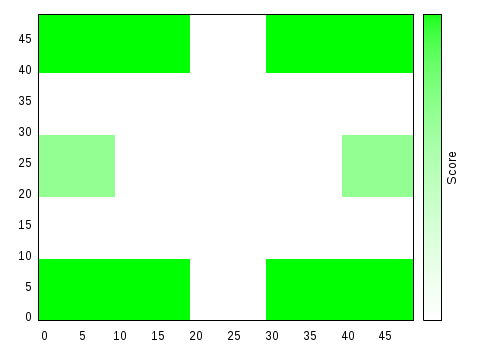
\includegraphics[scale=0.66]{ele.png}
\caption{Rozkład potencjału na elektrodach na wysokości $nz_2=15$ pudła obliczeniowego.}{\label{ele}}
\end{center}
\end{figure}
\section*{Wyniki}
Kroki siatki przyjmujemy $dx=dy=dz=10$ nm.
Rozmiary pudła przyjmujemy $nx=ny=50$. Położenie elektrod przedstawiono na rysunku \ref{ele}
(wysokość $nz_1=15$). Nasza studnia kwantowa znajduje się na wysokości $nz_2$. Obliczenia potencjału w środku studni
 wykonujemy dla kilku wartości $nz$ aby ustalić optymalną wysokość pudła. 
Wyniki przedstawiamy na wykresie \ref{w_nz}. Widzimy, że wartość potencjału nie zależy od rozmiarów pudła 
z dobrą dokładnością dla $nz=45$. Taką właśnie wartość przyjmujemy w dalszych obliczeniach. Sprawdzamy następnie dla ilu iteracji
zewnętrznych potencjał się stabilizuje (wykres \ref{w_N}). Widać, że dla $150$ wartość się już praktycznie nie zmienia. Dla takiej wartości
kroku sporządzamy wykresy potencjały wewnątrz studni (wykresy \ref{1} i \ref{2}).

\begin{figure}[h]
\begin{center}
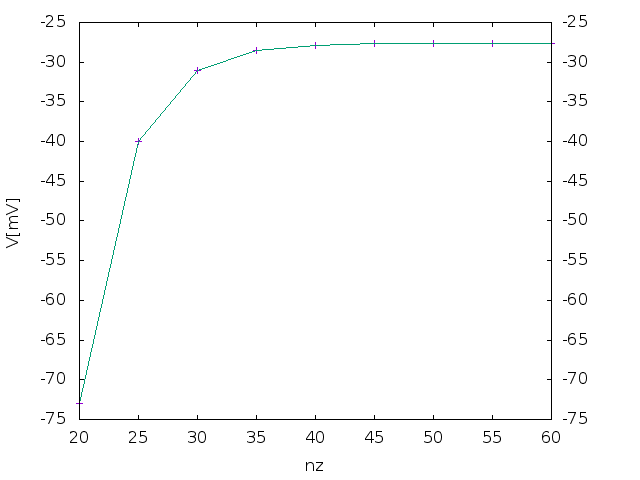
\includegraphics[scale=0.66]{nz.png}
\caption{Potencjał w centrum studni kwantowej w funkcji wysokości pudła obliczeniowego.}{\label{w_nz}}
\end{center}
\end{figure}
\begin{figure}[h]
\begin{center}
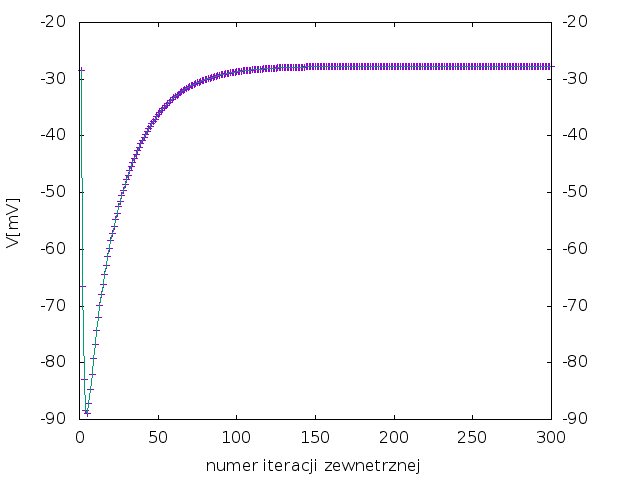
\includegraphics[scale=0.66]{numer.png}
\caption{Potencjał w centrum studni kwantowej a więc dla $nx/2$, $ny/2$, $nz_1=10$ w funkcji iteracji
zewnętrznej.}{\label{w_N}}
\end{center}
\end{figure}
\begin{figure}[h]
\begin{center}
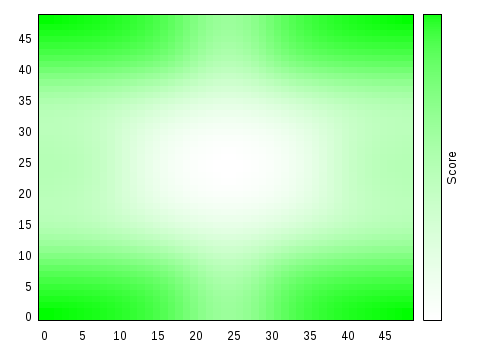
\includegraphics[scale=0.66]{2.png}
\caption{Rozkład potencjału w studni kwantowej wewnątrz nanourządzenia (wysokość $nz_1$). }{\label{2}}
\end{center}
\end{figure}
\begin{figure}[h]
\begin{center}
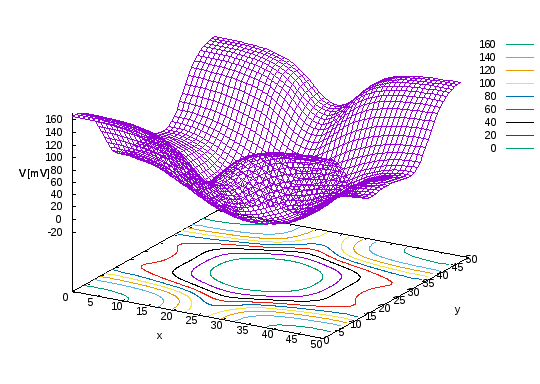
\includegraphics[]{1.png}
\caption{Rozkład potencjału w studni kwantowej wewnątrz nanourządzenia na wykresie trójwymiarowym (wysokość $nz_1$).}{\label{1}}
\end{center}
\end{figure}

\section*{Podsumowanie}
Przyjęte warunki brzegowe sprawiają, iż modelujemy pojedyncze urządzenie umieszczone w 
matrycy. Widzimy, że w zadanych warunkach (modelu urządzenia) powstaje studnia niskiego potecjału. Przy zadanych warunkach otrzymano studnię 
o głębokości rzędu 100 mV. To duża watrość biorąc pod uwagę, że elektrody naładowane były potencjałem poniżej 1V (względem podłoża).
\end{document}


